\documentclass{amcs}
\usepackage{verbatim}

\title[Implemention and evaluation...]{Implementation and evaluation of fine-tuning methods of PI controller with PLC-PID Tuner}

\author[ad1][]{Jakub MO\.{Z}ARYN}
\author[ad1][]{Damian SUSKI}
\author[ad1][]{Arkadiusz WINNICKI}


\correspondingauthor{First AUTHOR}

\address[ad1]{Institute of Automatic Control and Robotics\\ Warsaw University of Technology, Address ul. Sw. A. Boboli 8, 02-525, Warsaw, Poland\\ e-mail: \url{j.mozaryn@mchtr.pw.edu.pl}}


\Runauthors{F. Author \it{et al.}}
%\Runauthors{J. Doe}
%\Runauthors{J. Doe and M. John}

%PLEASE DO NOT MODIFY OR REMOVE THESE!
%\Year{}
%\Vol{}
%\No{}
%\Startpage{}
%\Endpage{}
%\DOI{}
%\Received{}
%\Revised{}
%\Rerevised{}
%\Accepted{}

\bibliographystyle{dcu}

\begin{document}
\begin{abstract}
In the paper, the method of an iterative modification of tuning parameters of a PI controller is presented. Proposed algorithms base on the off-line evaluation of quality indices. They were tested using PLC-PID Tuner - the application developed for tuning PID controller in S7 Simatic PLCs. It was shown that for some cases  proposed iterative method of modifying tuning parameters might increase the control quality. Furthermore, the gain margin and phase margin achieved  through this method are close to values recommended for  practical applications.
\end{abstract}

\begin{keywords}
keyword 1, keyword 2, \dots, keyword 5. Please provide a few keywords (3--5) and keep them specific.
\end{keywords}
\maketitle

\section{Introduction}
Despite all the progress in advanced control, the PID (proportional-integral-derivative) algorithm remains the most popular. Its gains are often chosen independently by an engineer, based on his experience or through some simple selection methods such as \textit{Ziegler-Nichols} \cite{Ziegler:1942} or \textit{Cohen-Coon} \cite{Cohen:1953}. However, regardless of the type of controlled process, there is usually requirement of exact response of the system. Without proper methodology of controller parameters tunig the quality of the control system may be unsatisfactory. Therefore many scientists and engineers develop tuning rules for different processes, where they consider different objectives. The survey presented in \cite{Odwyer:2006} gives the total of 1134 separate rules for PI and PID controllers. Such statistics were done in 2006, and one can expect that until now this number has increased significantly.

Nowadays, most of small and medium size production lines are controlled by Programmable Logic Controllers (PLC) which allow user to create the simple single loop control system as well as more complex structures. The main issue that ensures the correct functionality of the automation system is a proper adjustment of controller parameters. It should allow to minimize the deviation of the process variables from the desired output response, and therefore reduce the cost of the process due to the energy and material losses. 

In many practical situations, it is impossible to develop one's own tuning rules. Popularity of PLC controllers result in the need to implement appropriate tools that support user during controller tuning. Unlike automation systems based on dedicated controllers such as Distributed Control System (DCS), solutions based on PLC don't have such wide support in terms of integration and operation of control algorithms. 

Recently, manufacturers of automation systems develop advanced software tools that allow autotuning of PID controllers implemented in PLC's, using  proprietary algorithms based on relay or area auto-tuning methods \cite{Astrom:1995}, \cite{Yu:2006}, \cite{Trybus:2011}. Such modules which facilitate PID tuning are integrated within e.g. TIA Portal (Siemens), Automation Studio (B\&R) or TwinCAT (Beckhoff) software. However, implemented  methods don't allow designing control system in terms of specific performance indexes \cite{Bishop:2010}, \cite{Mozaryn:2013} e.g. gain and phase margin, integral of the squared error (ISE) or the integral of the absolute value of error (IAE). Therefore, it has limited use in processes which apart from minimizing standard indices, must meet additional criteria like sensitivity or robustness. 

Most applications that allow identification (e.g. IDCAD \cite{Janiszowski:2002}, MATLAB/Simulink, LabVIEW) don't have automatic procedures for tuning the specific controller, especially in industrial environment where the additional software is required to communicate with PLC to collect and archive values of the process variables. After process identification, controller parameters can be calculated   \cite{Odwyer:2009} and then implemented in PLC. Based on these premises the choice of proper method in industrial environment can be very complicated and time consuming. Therefore, the possibility to test, compare and use of wide variety of methods is very reduced. 

These facts were the inspiration to create PLC-PIDTuner application which combines above mentioned functionalities: real process data collection using Simatic S7 1200/1500 controllers, SISO system identification, tuning of PID controller parameters with different methods, verification of the control system in time and frequency domains using various performance indices. PLC-PIDTuner simplifies the tuning rule selection process and can be used by the field engineers with basic knowledge of control engineering.

The article is organized as follows. In section II, the implementation details of PLC-PIDTuner are described. Then, in section III, the PLC controller tuning methodology is presented. Section IV describes results obtained during exemplary verification of developed application, based on a model of the 3rd order lag system with delay. Finally, in section V further development ideas are presented and in section VI concluding remarks are given..

\section{Implementation details}
%
PLC-PIDTuner is based on the open and free standards. Application allows tuning of \texttt{PID\_Compact} function block implemented in SIMATIC S7-1200 and S7-1500 controllers which are relatively new products in Siemens SIMATIC S7 products line \cite{Mozaryn:2016}. 

In PLC-PIDTuner there are implemented numerous methods, supporting different stages of the control system design: 
%
\subsection{PID controller structure}

PLC-PIDTuner application considers PID algorithm implemented as follows:

\begin{equation}\label{eq20}
y(s)=K_{p}\left[1+\frac{1}{T_{i}s}+\frac{T_{d}s}{\frac{T_{d}}{k_{d}}s+1}\right]e(s)
\end{equation}

where: $K_{p}, T_{d}, T_{i}$ are proportional, derivative and integral gains, $k_{d}$ dynamic gain (during tests $k_{d}=6$). 

In \texttt{PID$\_$Compact} function block in S7-1200 PLC there is implemented PID controller in 2-DOF form \cite{Siemens:2013}:
%
\begin{equation}\label{eq21}
\begin{array}{ll}
y(s)=&K_{p}\left[(by_{\text{sp}}(s)-y(s))+\frac{1}{T_{i}\cdot s}(e_{\text{sp}}(s))+\right.\\
&\left.+\frac{T_{d}s}{aT_{d}s+1}(cy_{\text{sp}}(s)-y(s))\right]
\end{array}
\end{equation}
Where $a$, $b$, $c$, are scaling parameters, and \begin{equation}
e_{\text(sp)}=y_{\text{sp}}-y(k)
\end{equation}\label{eq23}

Equation (\ref{eq21}) can be converted into (\ref{eq20}) by setting parameters $a=1$, $b=1$, $c=1$. 
%
\subsection{Procedure of the controller parameters tuning with PLC-PIDTuner}
Presented application  divides controller tuning process into three main steps:

\begin{enumerate}
	\item STEP 1: Process identification.
	\item STEP 2: Calculation of the controller parameters.
	\item STEP 3: Verification of the control system performance in time and frequency domains.
\end{enumerate}

Thorough procedure divided into different sub-stages is presented in Fig. \ref{fig1}. Application contains simulation tools to verify the performance of the system in each sub-stage. Consequently, problems with the tuning process or decrease of an accuracy can be detected early and corrected. 

\begin{figure*}[!t]
	\centering
	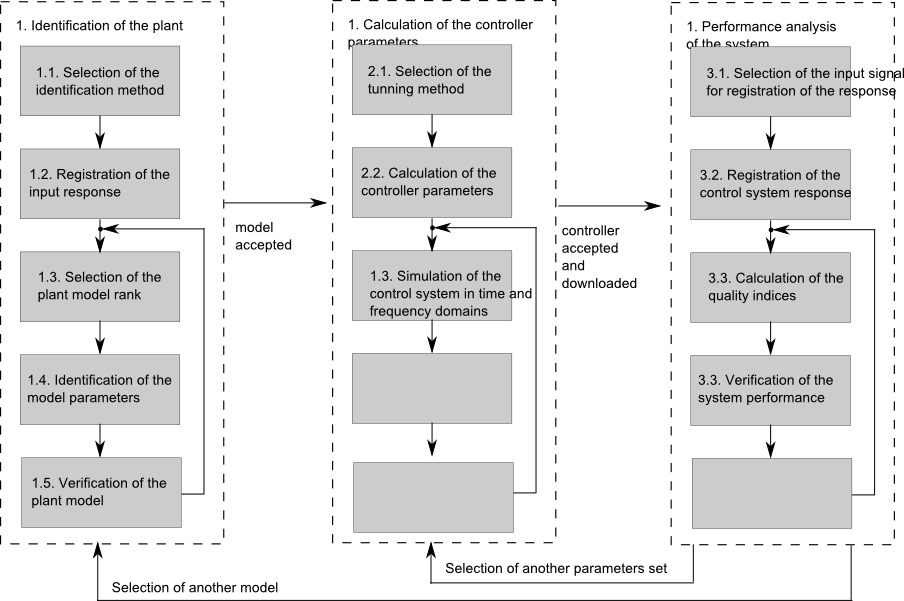
\includegraphics[width=1\textwidth]
	{Figure1}
	\caption{Procedure of PLC tuning process using PLC-PIDTuner.}
	\label{fig1}
\end{figure*}.

There is possibility to extend PLC-PIDTuner functionality by implementing identification methods, tuning methods and performance indices in standardized, separate DLL libraries. Such approach allows adapting the application to user needs based on expert knowledge of controlled industrial process. 

\subsection{Process identification}
%
The identification procedure provides mathematical model of process calculated on the basis of collected data of the control and process variables. It usually requires generation of proper excitation signal which affects industrial process and results in financial losses. Therefore, signal shape and parameters are often limited. PLC-PIDTuner allows coosing the suitable, least invasive excitation signal and set it's shape and parameters e.g. range of values or start/stop times of the step function.

In PLC-PIDTuner there are implemented following identification methods:
\begin{enumerate}
	\item secant method \cite{Haber:1999},
	\item tangent method \cite{Haber:1999},
	\item \textit{Strejc} method \cite{Strejc:1959},
	\item extended least squares (ELS) method  \cite{Mozaryn:2016}.
\end{enumerate}

Each method can be invoked in the application, and identified model parameters are saved for further controller tuning and process simulation. Moreover, user is able to select and compare several models identified by means of different methods. 

Secant, tangent and \textit{Strejc} methods are based on step response and specified mathematical model of the plant. Therefore they are mainly used for rough approximation of plant dynamics, which is often insufficient for the purpose of computer simulation or controller tuning. Therefore, ELS method is implemented, which is more accurate and easy in numerical implementation \cite{Mozaryn:2016}. 

PLC-PIDTuner allows user to compare determined model with the real plant by automatically calculating the response of the model. It allows verifying the quality of identified model using several indexes e.g. Integral Squared Error (ISE),  Integral Absolute Error (IAE), Integral Time-weighted Absolute Error (ITAE) and select the best of several models.

\subsection{Tuning of the controller parameters}
%
Tuning of the controller parameters is performed on the basis of the process model identified in previous stage. There are impemented over 750 tuning methods, classified into groups based on the model type \cite{Odwyer:2009}. Furthermore, user has the possibility to select proper tuning method in terms of:
%
\begin{itemize}
	\item control algorithm (P, PI, PD, PID),
	\item type of tuning method \cite{Odwyer:2009},
	\item minimization of specified quality index,
	\item additional options e.g. required overshoot.
\end{itemize}

The set of the methods and calculated parameters, can be further examined using  built-in time and frequency domains analysis modules. It should be emphasized, that all simulations are carried out with real PLC controller that communicates with PLC-PIDTuner.

Such functionality enables to choose the set of controller parameters more precisely. By modifying controller parameters and subsequently verifying control system response, user can adjust its properties to meet the control objectives. Furthermore, build-in simulation helps to verify designed control system without the need of costly experiments performed with the real process.
%
\subsection{Analysis of the control system performance}
%
After adjusting and downloading controller parameters, PLC-PIDTuner application allows user to verify operation of real control system. It is possible to plot and archive process variable values, change controller mode (Auto/Manual) or change set point value. Therefore, different quality indices in time domain can be calculated for the designed system. There were implemented 7 basic quality indices in time and frequency domain, described in detail in \cite{Kolaj:2015}.

Build-in PLC-PIDTuner module for analysis in frequency domain  allows operator to automatically draw \textit{Bode} and \textit{Nyquist} plots using simulation of the identified model. PLC-PIDTuner determines stability margins of the designed control system by calculating phase ($\Delta \phi$) and gain ($\Delta L$) margins \cite{Bishop:2010} \cite{Holejko:2012}. These values characterize the robustness of the control system to changes of the process parameters caused e.g. by aging of the actuators. 

On the basis of collected data PLC-PIDTuner automatically calculates values of selected quality indexes. It allows user to rate real control systems operation in terms of certain properties. If real control system does not meet the requirements, the steps of controller parameters  calculation or process mathematical model identification should be repeated.
%
\subsubsection{Time domain analisys}
%
The quality of the control system was analyzed in the time domain using following indexes: 
\begin{itemize}
	\item Maximum error 
	\begin{equation}
	e_{\text{sp}\max}=\max_{k}[e_{\text{sp}}(k)]
	\end{equation}\label{eq22}
	\item Overshoot 
	\begin{equation}
	\gamma=\left|\dfrac{e_2}{e_1}\right|100\%
	\end{equation}\label{eq24}
	where $e_1$ and $e_2$ are the first 2 consecutive biggest errors with opposite signs, assuming as the zero level (baseline) the steady state value of the output signal $y(t)$ after transient response.
	\item Transient response time $T_{R}$ - it is the time between the moment of change of the set point $y_{\text{sp}}(k)$, or introduction of disturbances $d(k)$ and the moment when error (\ref{eq22}) reaches a fixed value inside a boundary $|0.05 e_{\text{sp}\max}(k)|$. 
	\item Integral Squared Error 
	\begin{equation}
	\text{ISE}_{\text{sp}}=\sum_{k}[e_{\text{sp}}(k)]^{2} 
	\end{equation}\label{eq25}
	\item Integral of Absolute Value of Error 
	\begin{equation}
	\text{IAE}_{\text{sp}}=\sum_{k}|e_{\text{sp}}(k)| 
	\end{equation}\label{eq26}
\end{itemize}

\subsubsection{Frequency domain analysis}
%
In the next step, based on the simulation with model characterized by lowest indices, stability margins of the designed control systems are calculated. Gain margin determines how much the magnitude of the control system should increase, to make it unstable. Control systems with sufficiently large gain margin and phase margin are robust to changes in the parameters of the object and external distortions. Knowledge of the stability margins values allow also to adjust controller parameters in order to improve quality in the time domain \cite{Mozaryn:2013}.   
%
\section{Fine-tuning of PID controller}
%
Desired control system, was characterized by following properties:

\begin{itemize}
\item \textbf{Property 1:} Short $T_{R}$ of the step response.
\item \textbf{Property 2:} Short $T_{R}$  after abrupt occurrence of disturbances.
\item \textbf{Property 3:} Output signal should have no visible high-frequency oscillations.
\end{itemize}

To specify the robustness of the system there should be performed analysis in the frequency domain. In PLC-PID Tuner are calculated gain margin and phase margin of the control system \cite{Mozaryn:2016}. Gain margin determines how much the magnitude of the control system should increase, to make it unstable. Control systems with sufficiently large gain margin and phase margin are robust to changes in the pa-rameters of the object and external distortions. If $\Delta M$  and $\Delta \phi$ decrease, the control system has transient oscillatory character and the overshoot, but also has short transient response time. 

In the proposed heuristic iterative modification procedures we propose to reduced chosen controller settings in order to comply with the following assumptions:

\textbf{Assumption 1:} Step response overshoot should be less than 5 \%.

\textbf{Assumption 2:} The change of $\Delta M$  should be less than 25\% of the original value and $\Delta \phi$ should be less than 25\% of the original value. 

Proposed PID fine-tuning iterative procedure can be presented in the form of algorithm as follows:

\begin{algorithm}[!h]
	\caption{FT1 - Iterative modification of the proportional gain}
	\label{a:alg1}
	\textbf{Step 1.} Set the iteration step $k=0$ . Enter the pre-tuned set of PID settings: $k_{p0}$, $T_{I0}$, $T_{D0}$, perform the step response experiment. Calculate and save values: $\gamma_{0}$, $\Delta M_{0}$, and $\Delta \phi_{0}$. Set $k_{p,0}=k_{p0}$. If $\gamma_{0}<5\%$ go to step 2, else go to step 6. 
	
	\smallskip
	\textbf{Step 2.} Set $k=k+1$, and $k_{p,k}=1,05k_{p,k-1}$  .
	
	\smallskip
	\textbf{Step 3.} Perform step response experiment, calculate values $\gamma_{k}$, $\Delta M_{k}$, and $\Delta \phi_{k}$.
	
	\smallskip
	\textbf{Step 4.} If $\gamma_{k}<5\%$, go to step 5, else go to step 6.
	
	\smallskip
	\textbf{Step 5.} If $\Delta M_{k}<(1\pm0,3)M_{0}$  and $\Delta \phi_{k}<(1\pm0,3)\phi_{0}$  go to step 2, else go to step 6.
	
	\smallskip
	\textbf{Step 6.} Set $k_{p}=k_{p,k-1}$ .
	
	\smallskip
	\textbf{Step 7.} Stop the algorithm.
\end{algorithm}

\begin{algorithm}[!h]
	\caption{FT 2 - Iterative modification of the integral gain}
	\label{a:alg1}
	\textbf{Step 1.} Set the iteration step $k=0$ . Enter the pre-tuned set of PID settings: $k_{p0}$, $T_{I0}$, $T_{D0}$, perform the step response experiment. Calculate and save values: $\gamma_{0}$, $\Delta M_{0}$, and $\Delta \phi_{0}$. Set $T_{I,0}=T_{I0}$. If $\gamma_{0}<5\%$ go to step 2, else go to step 6. 
	
	\smallskip
	\textbf{Step 2.} Set $k=k+1$, and $T_{i,k}=0,95 T_{I,k-1}$  .
	
	\smallskip
	\textbf{Step 3.} Perform step response experiment, calculate values $\gamma_{k}$, $\Delta M_{k}$, and $\Delta \phi_{k}$.
	
	\smallskip
	\textbf{Step 4.} If $\gamma_{k}<5\%$, go to step 5, else go to step 6.
	
	\smallskip
	\textbf{Step 5.} If $\Delta M_{k}<(1\pm0,3)M_{0}$  and $\Delta \phi_{k}<(1\pm0,3)\phi_{0}$  go to step 2, else go to step 6.
	
	\smallskip
	\textbf{Step 6.} Set $T_{I}=T_{I,k-1}$ .
	
	\smallskip
	\textbf{Step 7.} Stop the algorithm.
\end{algorithm}

\section{Expemental verification}

\subsection{Control system structure}
%
The process was controlled in closed-loop control system, presented in Fig. 2.

In the control system (Fig. 2), an output of the process   is the liquid level in the tank Z1 (H1). It is compared with the desired output response (setpoint)   and an output error is given as:
\begin{equation}
e(t)=y(t)-w(t)
\end{equation}
The error (1) is used by the controller to adjust the control signal   which, through an actuator (pump) affects the regulated process. In the system there are disturbances   (leakage) which can be introduced, as it is described in chapter 2.

The control algorithm was implemented on a Siemens S7-1200 PLC controller. 

\subsection{Identification of the control plant}

\subsection{Selection of PID controller parameters}
%
\subsection{Pre-tuning of PID controller}
In \cite{Odwyer:2009} there are described 1731 different types of PID tuning rules, so the proper criteria should be used to choose the most suitable settings. Tuning rules selection (pre-tuning) criteria were as follows:
%
\begin{itemize}
\item a) Type of a process (stationary or nonstationary).
\item b) Model of the process.
\item c) PID controller structure.
\item d) The ratio of transport delay and the time constant of the process:
\begin{equation}
R=\dfrac{T_{d}}{T_{z}}
\end{equation}
\end{itemize}

\subsection{Fine-tuning of PID controller}

Obtained quality indices after the iterative modifications (FT1 and FT 2), are gathered in Table 2.

\section{Conclusions}

\begin{acknowledgment}
Please acknowledge here all and any support, institutional or individual, which you have received for your work.
\end{acknowledgment}

\bibliography{amcs_pid}

\begin{biography}[photo]{Jakub Mo\.{z}aryn.}Place a brief biography here xxx xxx xxxxx xx xxx xxx xxx xx xxxx xx xxxxxxx xxx xxx xx xx xx xxxxx xx xxxx xxx xxx xxxxx xx xxx xxx xxx xx xxxx xx xxxxxxx xxx xxx xx xx xx xxxxx xx xxxx xxx xxx xxxxx xx xxx xxx xxx xx xxxx xx xxxxxxx xxx xxx xx xx xx xxxxx xx xxxx xxx xxx xxxxx xx xxx xxx xxx xx xxxx xx xxxxxxx xxx xxx xx xx xx xxxxx xx xxxx xxx xxx xxxxx xx xxx xxx xxx xx xxxx xx xxxxxxx xxx xxx xx xx xx xxxxx xx xxxx xxx xxx xxxxx xx xxx xxx xxx xx xxxx xx xxxxxxx xxx xxx xx xx xx xxxxx xx xxxx xxx xxx xxxxx xx xxx xxx xxx xx xxxx xx xxxxxxx xxx xxx xx xx xx xxxxx xx xxxx.
\end{biography}

\begin{biography}[]{Damian Suski.}Place a brief biography here xxx xxx xxxxx xx xxx xxx xxx xx xxxx xx xxxxxxx xxx xxx xx xx xx xxxxx xx xxxx xxx xxx xxxxx xx xxx xxx xxx xx xxxx xx xxxxxxx xxx xxx xx xx xx xxxxx xx xxxx xxx xxx xxxxx xx xxx xxx xxx xx xxxx xx xxxxxxx xxx xxx xx xx xx xxxxx xx xxxx xxx xxx xxxxx xx xxx xxx xxx xx xxxx xx xxxxxxx xxx xxx xx xx xx xxxxx xx xxxx xxx xxx xxxxx xx xxx xxx xxx xx xxxx xx xxxxxxx xxx xxx xx xx xx xxxxx xx xxxx xxx xxx xxxxx xx xxx xxx xxx xx xxxx xx xxxxxxx xxx xxx xx xx xx xxxxx xx xxxx xxx xxx xxxxx xx xxx xxx xxx xx xxxx xx xxxxxxx xxx xxx xx xx xx xxxxx xx xxxx.
\end{biography}

\begin{biography}[]{Arkadiusz Winnicki.}Place a brief biography here xxx xxx xxxxx xx xxx xxx xxx xx xxxx xx xxxxxxx xxx xxx xx xx xx xxxxx xx xxxx xxx xxx xxxxx xx xxx xxx xxx xx xxxx xx xxxxxxx xxx xxx xx xx xx xxxxx xx xxxx xxx xxx xxxxx xx xxx xxx xxx xx xxxx xx xxxxxxx xxx xxx xx xx xx xxxxx xx xxxx xxx xxx xxxxx xx xxx xxx xxx xx xxxx xx xxxxxxx xxx xxx xx xx xx xxxxx xx xxxx xxx xxx xxxxx xx xxx xxx xxx xx xxxx xx xxxxxxx xxx xxx xx xx xx xxxxx xx xxxx xxx xxx xxxxx xx xxx xxx xxx xx xxxx xx xxxxxxx xxx xxx xx xx xx xxxxx xx xxxx xxx xxx xxxxx xx xxx xxx xxx xx xxxx xx xxxxxxx xxx xxx xx xx xx xxxxx xx xxxx.
\end{biography}

\end{document}
